\chapter{SYSTEM ARCHITECTURE}

\section{OVERVIEW}

Stockify uses a three-tier architecture (presentation, application, data) focused on scalability, security, and maintainability.

\section{ARCHITECTURAL DESIGN}

\begin{itemize}
    \item Presentation: React frontend (responsive UI)
    \item Application: Node.js + Express REST API
    \item Data: MongoDB Atlas (document store)
\end{itemize}

\subsection{System Architecture Diagram}

The system follows a layered architecture with clear separation of concerns across presentation, application, and data layers.

\begin{figure}[H]
    \centering
    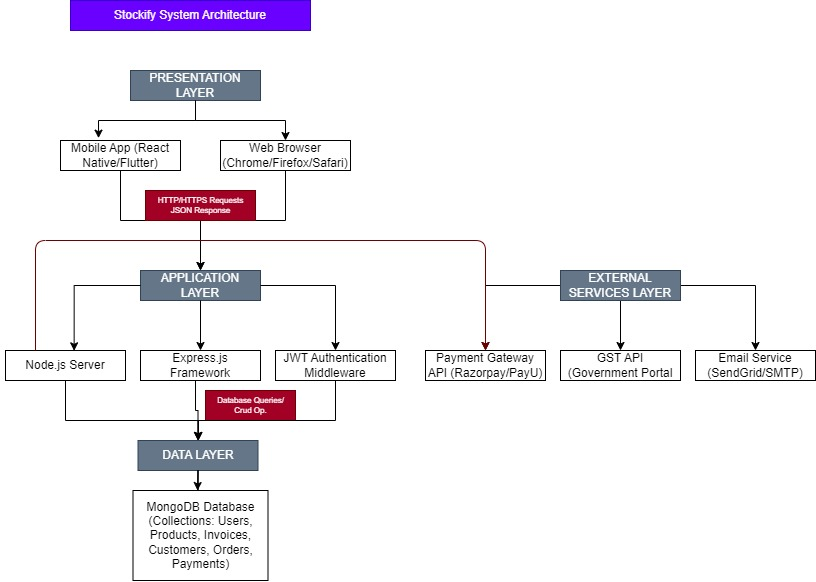
\includegraphics[width=0.85\textwidth]{assets/screenshots/System Architecture.jpg}
    \caption{Three-tier system architecture of Stockify}
    \label{fig:system-architecture}
\end{figure}

The architecture diagram illustrates the complete flow from user interfaces through the application layer to the database. The presentation layer consists of mobile and web applications communicating via HTTP/HTTPS with the application layer. The application layer comprises the Node.js server, Express.js framework, and JWT authentication middleware, which handle business logic and API endpoints. Database queries and CRUD operations connect the application layer to MongoDB Atlas in the data layer, storing all collections including Users, Products, Invoices, Customers, Orders, and Payments. External services such as payment gateways, GST API, and email services integrate at the application layer.

\section{USE CASE DIAGRAM}

The use case diagram represents the functional requirements and interactions between different user roles and the system.

\begin{figure}[H]
    \centering
    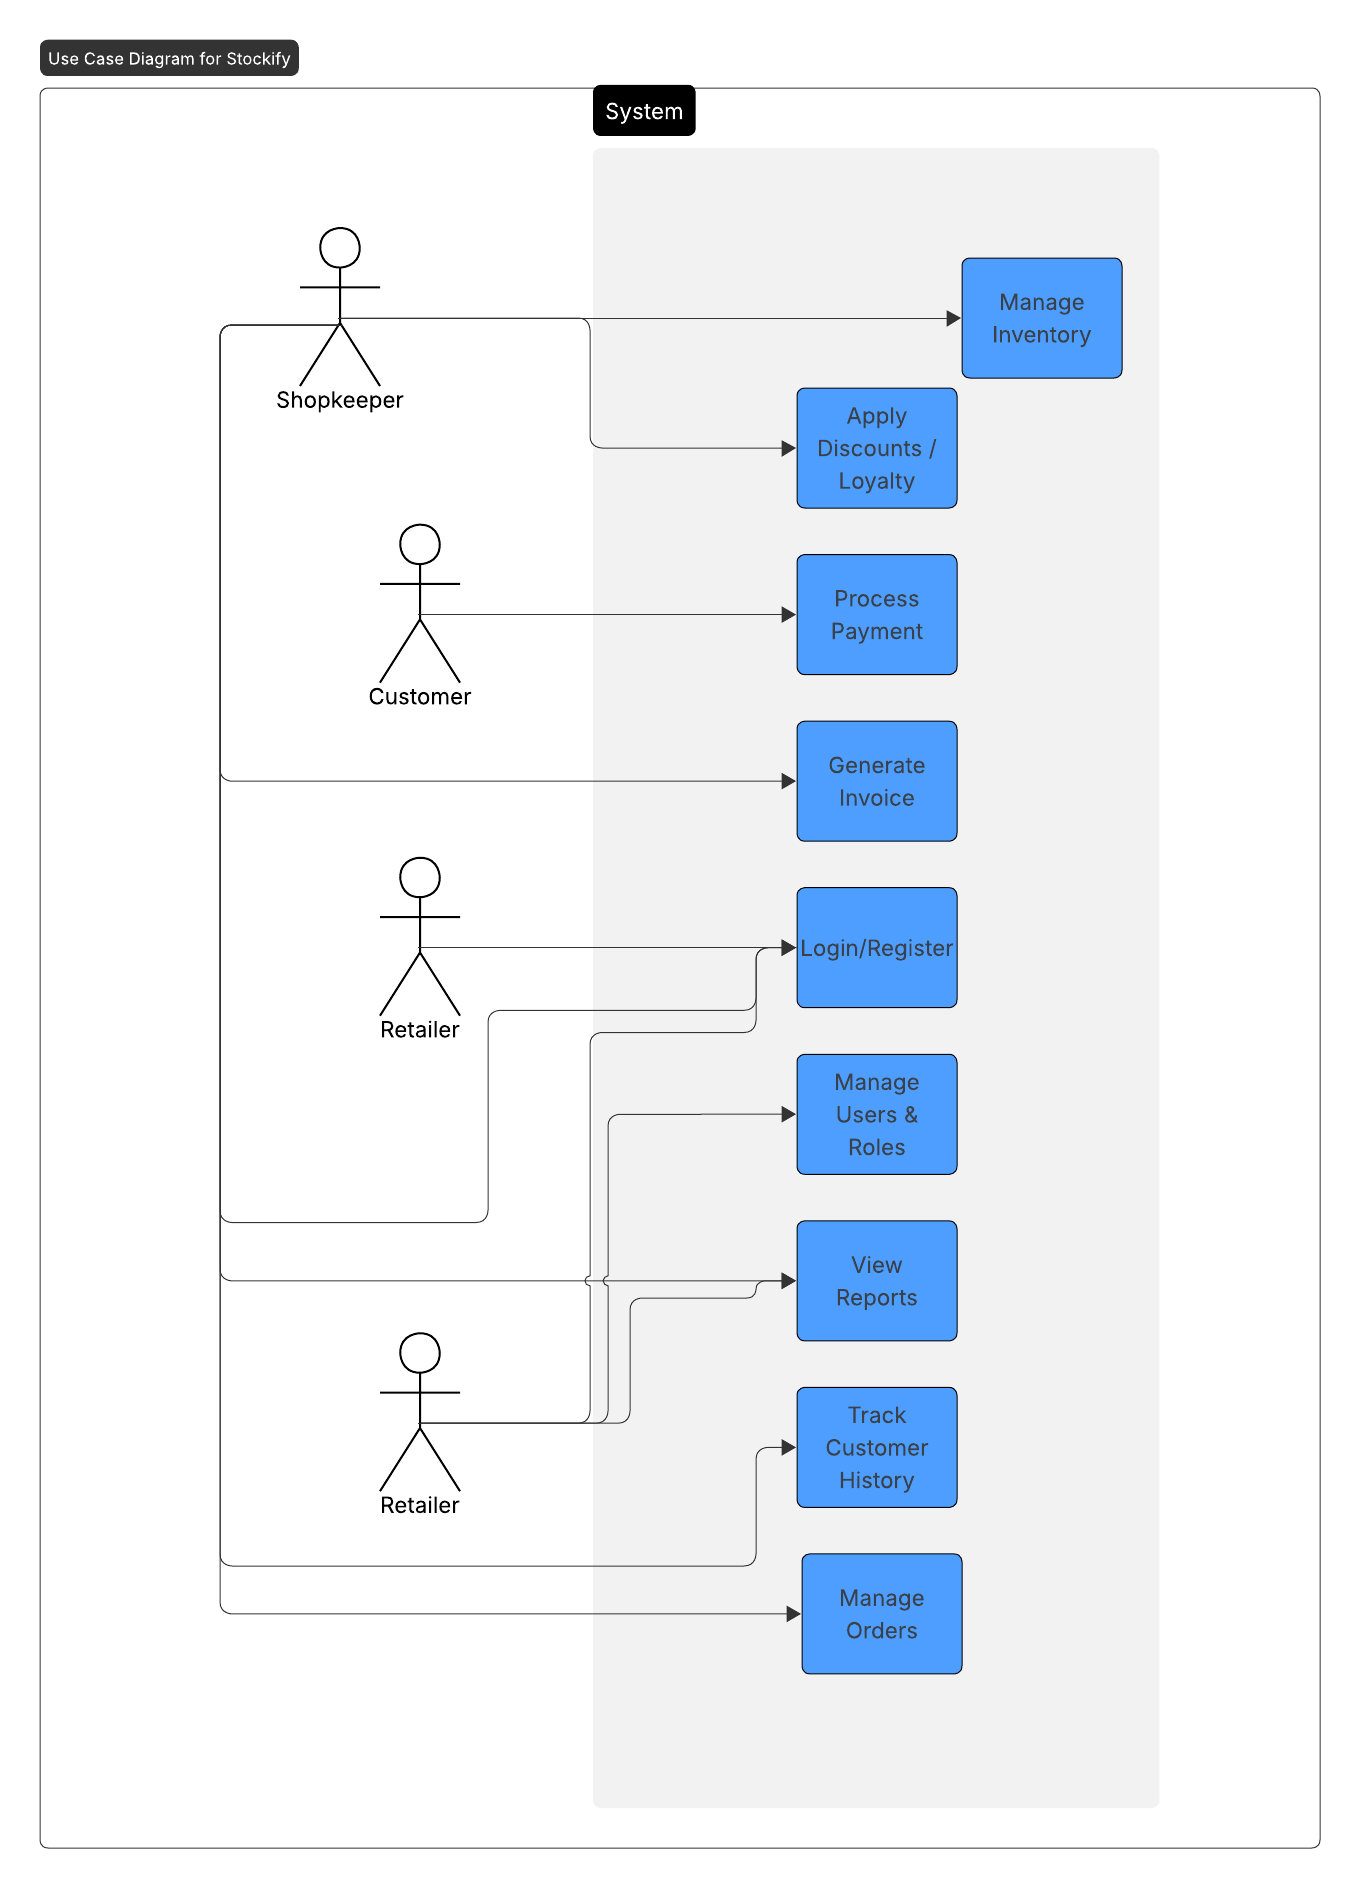
\includegraphics[width=0.9\textwidth]{assets/screenshots/Use Case.png}
    \caption{Use case diagram showing user interactions with Stockify}
    \label{fig:use-case}
\end{figure}

The system supports multiple user roles with distinct capabilities:

\begin{itemize}
    \item \textbf{Shopkeeper}: Manages inventory, applies discounts and loyalty programs
    \item \textbf{Customer}: Processes payments and generates invoices
    \item \textbf{Retailer}: Performs login/registration, manages users and roles, views reports, tracks customer history, and manages orders
\end{itemize}

These use cases define the core functionality required for effective inventory management and billing operations.

\section{FRONTEND ARCHITECTURE}

The frontend follows a pages/layouts/components pattern. State is managed with React Context for auth, local state for UI, and custom hooks for data fetching. Data flows from user actions → API calls → state updates → UI render.

\section{BACKEND ARCHITECTURE}

The backend uses an MVC-like structure: Mongoose models, controllers for business logic, routes for endpoints, and services for shared functionality. Middleware handles auth (JWT), validation (Joi), errors, logging, and security.

\section{DATABASE ARCHITECTURE}

MongoDB is used for flexible document modeling, aggregation queries, and horizontal scaling. Tenant isolation relies on a `createdBy` field and tenant-aware queries with appropriate indexes. Key collections: Users, Products, Sales, Categories, Customers, Suppliers.

\section{SECURITY}

Authentication: JWT and Google OAuth; passwords hashed with bcrypt. Authorization uses role checks and resource ownership validation. Standard protections (Helmet, CORS, input validation) are applied.

\section{PERFORMANCE}

Frontend: code-splitting, lazy loading, and asset caching. Backend: indexing, connection pooling, caching frequent responses, and efficient pagination.

\section{DEPLOYMENT}

Dev: Vite (5173), Node with nodemon (5000), Atlas connection. Prod: static frontend build, Node.js managed process (PM2), Atlas backups, HTTPS and load balancing.

\section{MONITORING \& INTEGRATION}

Centralized logging, performance metrics, health checks, and integrations (Google OAuth, email, storage, analytics) support operations and observability.

\section{SCALABILITY}

Designed for stateless API scaling, Atlas scaling, CDN-backed static assets, and load balancers to handle growth.

\section{CONCLUSION}

The architecture provides a modular, scalable foundation that supports secure multi-tenant operation and future enhancements.